\documentclass[12pt]{article}
\usepackage[utf8]{inputenc}
\usepackage[brazil]{babel}
\usepackage{sbc-template}
\usepackage{graphicx,url}
\usepackage[table,xcdraw]{xcolor}
\usepackage{longtable}

\sloppy

\title{Mestrado em Informática\\ Proposta de Trabalho \\ Analise de dados para verificar a viabilidade de Startups Tecnlógicas na área de tecnologia}

\author{Ricardo Moraes Guimarães\inst{1}}


\address{Universidade Federal do Amazonas - UFAM\\
\email{ricardommoraes@gmail.com}
}

\begin{document}

\maketitle

\section{Introdução} \label{sec:intro}

Atualmente, as universidades brasileiras estão investindo um esforço considerável para incorporar uma nova missão, a de que não é apenas formar recursos humanos na fronteira do conhecimento, mas fazer com que esses recursos sejam capazes de traduzir conhecimento na forma de novos negócios e ou produtos, processos e serviços. Além de mencionar mais uma missão das universidades, o autor \cite{hannon2013entrepreneurial:2013} ao citar \cite{gibb2012exploring:2012}, menciona que é preciso criar, dentro das universidades ambientes mais propícios para o desenvolvimento de mentalidades e comportamentos empreendedores, é importante que as próprias universidades possam pensar estrategicamente de forma mais empreendedora.

Juntamente com essa missão, estão as politicas de CT\&I no que tange a criação de novas incubadoras e parques tecnológicos. Em conjunto, espera-se que essas políticas gerem impactos de natureza econômica, tais como aumento de oferta de empregos qualificados e de produtos com maior valor agregado e com maior potencial de competitividade internacional \cite{hannon2013entrepreneurial:2013}.

Segundo \cite{dimitriadis2008opinia:2008}, conforme citado por \cite{staniewski2015motivating:2015}, muitos estudos mostram que o empreendedorismos tem papel importante no desenvolvimento social e econômico. Influenciando no crescimento econômico, na criação de melhores lugares de trabalho, melhoria na produtividade da força de trabalho, contribui ainda para a criação de novas tecnologias, bens e serviços e aumenta a concorrência no mercado local.

E para o caso da região norte, e mais especificamente, para a área de influência do Polo Industrial de Manaus, esse fenômeno tem como importância estratégica o aumento da inovação e o progresso tecnológico \cite{hannon2013entrepreneurial:2013}. E neste sentido, a indústria de software desempenha um papel primordial, visto que, além de não ter impacto ambiental, por não consumir recursos naturais, ela é pouco ou nada dependente de infraestrutura logística, demandando apenas conexão de Internet estável. Além disso, a indústria de software é tipicamente de alto valor agregado, promovendo impacto econômico sem a necessidade de uma força de trabalho intensa, o que seria um problema em uma região com baixa densidade populacional.

Apesar das vantagens relacionadas com a criação de empresas de software de base tecnológica para a região norte serem discutidas a muitos anos \cite{bergerman2002}, as dificuldades enfrentadas pelo jovem empreendedor ainda são muitas. Desde falta de conhecimento de como iniciar uma empresa, até as diversas inseguranças jurídicas intrínsecas a um Brasil burocrático e acostumado a um capitalismo de compadrio.

Torna-se, portanto, necessário construir um corpo de conhecimento para que o empreendedor possa desenvolver sua iniciativa com a maior autonomia possível, bem como encontrar rapidamente os caminhos necessários para o desenvolvimento estratégico do seu negócio. E acreditando que um melhor caminho é a promoção de um ambiente inovador e que seja ao mesmo tempo cheio de possibilidades, mas, e principalmente, autônomo. 

Neste sentido, um vasto número de manuais foram escritos que tratam de forma mais especifica de diferentes aspectos do desenvolvimento de novos negócios e que fornecem consideráveis conselhos práticos sobre com uma empresa pode aumentar suas chances de sobrevivência e sucesso \cite{davidsson2003business:2003}. Porém, eles não tratam adequadamente os aspectos locais de um ecossistema onde a conhecida hélice-tripla não funciona com o passo sincronizado. Com isso, o presente trabalho tem como intuito responder a uma pergunta crítica:

Como a cultura molda a percepção individual em relação às barreiras para empreender e em relação às intenções para se tornar um empreendedor acadêmico dentro do contexto da indústria de software de base tecnológica?

Para esta proposta, será feito uma pesquisa baseado no modelo \textbf{Businnes Platform Model} proposto por \textit{Magnus Klofsten}, a fim de avaliar a percepção de cada empreendedor em relação às barreiras para empreender e em relação às intenções para se tornar um empreendedor acadêmico.

Se o empreendedorismo produz tantos benefícios, parece essencial explorar os fatores que poderiam facilitar ou dificultar o início da própria atividade comercial \cite{staniewski2015motivating:2015}.

\section{Objetivos} \label{sec:objec}

Neste trabalho, buscaremos responder ao questionamento que estimulou o desenvolvimento deste projeto  baseado no modelo \textbf{Businnes Platform Model} proposto por \textit{Magnus Klofsten}, a fim de avaliar a percepção de cada empreendedor tecnológico em relação às barreiras para empreender e em relação às intenções para se tornar um empreendedor acadêmico.

\begin{itemize}
	\item{Elaborar e desenvolver métricas para a análise e uso de informações, aplicados em \textit{startup} tecnológicas.}
	\item{Elaborar surveys para coleta de dados das \textit{startups} incubadas.}
	\item{Aplicar o modelo de \textit{Magnus Klofsten} nas informações coletadas a partir de survey e pesquisas na \textit{web}.}
	\item{Utilizar técnica de estração de dados textual aplicado ao princiapl componente analisado (PCA).}
	\item{Desenvolver sistema de recomendação, baseado no modelo \textbf{Businnes Platform Model} proposto por \textit{Magnus Klofsten}.}
\end{itemize}

\section{Metodologia} \label{sec:Metod}

Esta pesquisa exploratótia utilizará como modelo de analise o método desenvolvido por \textit{Magnus Klofsten}, onde, a partir de oito pilares determinar o processo incial de desenvolvimento de uma empresa. Esses oito pilare são fundamentalmente a ideia de negócio, produto, mercado, organização, experiência do grupo, grupo com o mesmo objetivo/motivação, relações com o cliente e outras relações, que compõem o modelo da plataforma de negócios. O objetivo dos 8 pilares é descrever o processo de desenvolvimento de uma \textit{startup} tecnológica de forma holística para a região norte. \cite{davidsson2003business:2003}.

O aumento do uso e popularidade da internet nos trouxe acesso livre a varios tipos de informações de produtos, pessoas, empresas, comércios entre outros. Essas mudanças transformaram a \textit{web} em um imenso repositório de informações para todos. Pesquisas relacionadas com geração de conhecimento a partir de informações extraídas dessas fontes públicas e acessíveis de dados são muito úteis e rica em informações \cite{liu:11}.

Será utilizado nessa pesquisa, dados coletados em sites das empresas imcubadas no ICOMP-UFAM, no CDTEC-UFAM e da incubadora do IFAM e do IDSM além de coletas realizadas com a utilização de survays na busca por padrões que possam ser medidos a partir do modelo de \textit{Magnus Klofsten}, com o intuíto de elaborar recomendações.

\section{Contextualização Bibliográfica} \label{sec:Contex. Bibli}
\subsection{The Business Platforme Model}
Segundo \cite{davidsson2003business:2003}, \textbf{Business Platform Model} foi publicada em 1992 e ao longo dos anos vem sofrendo melhorias. A idéia central do \textbf{Businnes Platform Model} é a análise e avaliação de uma empresa através da investigação de 8 diferentes princípios, sendo esses princípio interligados afim de stabelecer uma visão geral do potencial e das possibilidades de sobrevivência da \textit{startup}. Esse modelo busca também orientar a identificação de áreas de melhoria em uma empresa, auxiliando seus lideres nas tomadas de decisões. Na figura a baixo pode-se identificar as 8 pedras angulares ou pilares, descritos no modelo \textbf{Businnes Platform Model}.

\begin{figure}[!ht]
\begin{center}
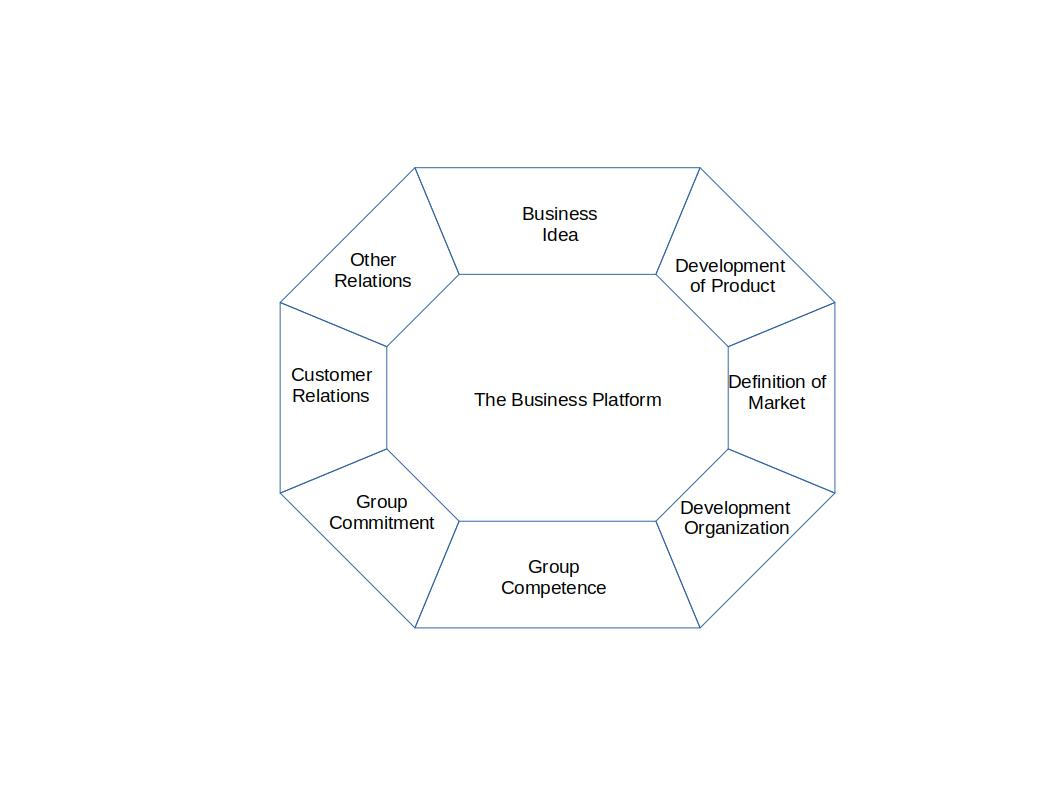
\includegraphics[scale=0.3]{cornerstones.jpg}
\caption{The Business Platforme Model-Cornerstones}
\pagebreak
\clearpage
\newpage
\end{center}
\end{figure}

A ideia fundamental deste modelo é que as empresas são vulneráveis em seu tempo de vida e continuamente correm risco de desaparecer no mercado. O sucesso da empresa é determinado pelo quão bem esta vulnerabilidade é superada.

\subsection{Empreendedorismos nas Universidades}
Para \cite{etzkowitz2002networks}, as universidades dependem da motivação dos acadêmicos para se envolverem em atividades empresariais de inovação com o mundo externo, a fim de cumprir sua missão de se tornar uma "universidade empreendedora". Na literatura, um empresário acadêmico é reconhecido de forma diferente de um empreendedor acadêmico. Um empreendedor acadêmico geralmente descreve como um acadêmico que se dedica a atividades de comercialização que muitas vezes resultam em criação de patentes, vendas de licenças ou criação de novos empreendimentos e empresas de spin out \cite{jensen2001proofs}. Enquanto que o empresário acadêmico é considerado como participante de uma ampla gama de atividades, colaboração e transferência de conhecimento, ligando a universidades com outras organizações.

Há vários estudos que identificam multiplas e muitas vezes conflitantes demandas de uma empreendedor acadêmico e dada a distância considerável entre a industria e as fronteiras do conhecimento acadêmico. A ideia é que haja um menor esforço para desenvolver solidos realacionamentos de colaboração a fim de gerar sucesso nos empreendimentos \cite{rothaermel2007university}.

Nos últimos anos, sugeriu-se que o modelo da hélice-tripla tenha desencorajado os fluxos de conhecimento e envolvimento entre universidades, industria e governo, a partir de inúmeros estudos que exploraram o envolvimento dos interessados nos conceitos que envolviam a hélice-tripla no final do século XX \cite{sperrer2016concept}. 

No entanto as críticas quanto ao modelo da hélice-tripla, juntamente com muitas universidades com desempenho inferior em termos de inovação, levaram a relatórios governamentais recentes onde é enfatizado a necessidade de as universidades aderirem a um maior envolvimento com a indústria e os clientes dentro de um ecossistema de hélice-quádruplo \cite{witty2013encouraging}.

\section{Cronograma} \label{sec:Crono}

\begin{longtable}[c]{|l|l|l|l|l|l|l|}
\caption{Cronograma} \label{my-label}\\ \hline
\endfirsthead
\endhead
\multicolumn{1}{|c|}{\textbf{Primeiro Ano}} & \multicolumn{6}{c|}{\cellcolor[HTML]{ECF4FF}Meses} \\ \hline
\rowcolor[HTML]{ECF4FF} 
\textbf{Atividades} & 1-2 & 3-4 & 5-6 & 7-8 & 9-10 & 11-12 \\ \hline
Cursar Disciplinas & \cellcolor[HTML]{C0C0C0} & \cellcolor[HTML]{C0C0C0} & \cellcolor[HTML]{C0C0C0} & \cellcolor[HTML]{C0C0C0} & \cellcolor[HTML]{C0C0C0} & \cellcolor[HTML]{C0C0C0} \\ \hline
Levantamento Bibliográfico & \cellcolor[HTML]{C0C0C0} & & & & & \\ \hline
Estudo do Problema & & \cellcolor[HTML]{C0C0C0} & \cellcolor[HTML]{C0C0C0} & & & \\ \hline
Definição da Metodologia & & & & \cellcolor[HTML]{C0C0C0} & \cellcolor[HTML]{C0C0C0} & \\ \hline
Defesa da Proposta de Dissertação & & & & & \cellcolor[HTML]{C0C0C0} \\ \hline
\multicolumn{1}{|c|}{\textbf{Segundo Ano}}  & \multicolumn{6}{c|}{\cellcolor[HTML]{ECF4FF}Meses} \\ \hline \rowcolor[HTML]{ECF4FF} 
\textbf{Atividades} & 1-2 & 3-4 & 5-6 & 7-8 & 9-10 & 11-12 \\ \hline
Validação da Metodologia & \cellcolor[HTML]{C0C0C0} & \cellcolor[HTML]{C0C0C0} & \cellcolor[HTML]{C0C0C0} & & & \\ \hline
Elaboração da Dissertação & & & \cellcolor[HTML]{C0C0C0} & \cellcolor[HTML]{C0C0C0} & \cellcolor[HTML]{C0C0C0} & \\ \hline
Defesa da Dissertação & & & & & & \cellcolor[HTML]{C0C0C0} \\ \hline
\end{longtable}

\newpage
\bibliographystyle{sbc}
\bibliography{proposta}

\end{document}